In this chapter, we build a complete picture of the Methodology applied during the subject research. We briefly analyze the dataset used and describe all components of the implemented model.

\section{Data Analysis and Exploration} \label{sec:data_analysis}

The dataset selected for sourcing the prediction model was part of the NeurIPS2021 Traffic4cast competition \cite{pmlr-v176-eichenberger22a}. This dataset consists of 360 days of data from 8 different cities with similar sizes derived from trajectories of a fleet of probe vehicles. The original data has 180 days from 2019 and another 180 days from 2020, as one of the questions of the challenge was to asses how the COVID pandemic affected traffic in different cities. As this represents a shift in the temporal distribution of the data, we choose not to use the 2020 half of it, intending to have an assumed temporal invariant distribution. Table\ref{tab:cities} disposes of all cities available on the dataset and the number of data points each city contains.

\begin{table}[!h]
\centering
\begin{tabularx}{\textwidth}{Xcc}
\hline
City & \# days & \# snapshots per day \\ \hline
Antwerp & 180 & 240 \\
Bangkok & 180 & 240 \\
Barcelona & 180 & 240 \\
Berlin & 180 & 240 \\
Chicago & 180 & 240 \\
Istanbul & 180 & 240 \\
Melbourne & 180 & 240 \\
Moscow & 180 & 240 \\ \hline
\end{tabularx}
\caption{List of the cities available on the dataset}
\label{tab:cities}
\end{table}

For a given time snapshot, the data of one city can be represented by a tensor of size $(495, 436, 8)$, where $495\times436$ represents the city grid, and $8$ stands for the channels, or pieces of information, per cell. These channels contain information on the volume and mean speed of the probe cars heading in the four diagonal directions. All data was normalized and discretized in the \texttt{uint8} range.

To better understand the data, distribution, and characteristics, the following analysis is conducted on the 5-minute snapshot that started at 12:00 on 9 January 2019 in Melbourne. Figures \ref{fig:speed} and \ref{fig:volume} show the distribution of values for both the speed (odd channels) and the volume (even channels). Notice the logarithmic scale on the $y$ axis. It's clear that while the volume has a more even distribution for non-zero values, there remains a massive bias for the zero values, as they represent more than 99\% of the data points. This indicates that most of our data comprises zeros and that activity should be treated as a rare event.

Furthermore, Figure \ref{fig:heatmap} confirms this theory, as it can be seen that most of the data for the speed channels is zero, and the volume, despite being better distributed, is also defined by a majority of zeros. Table \ref{tab:data_analysis} shows the statistics for each channel and reinforces the proposed thesis.



\begin{figure}[!ht]
    \centering
    \begin{minipage}{0.45\textwidth}
        \centering
        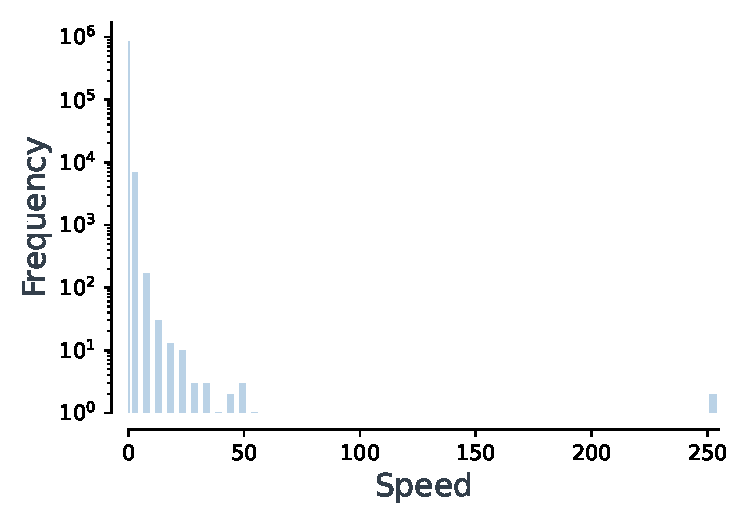
\includegraphics[width=0.9\textwidth]{./figures/speed.pdf}
         \caption{Histogram for data distribution for the speed. Note the first (very thin) bin with the null values.}
         \label{fig:speed}
    \end{minipage}\hfill
    \begin{minipage}{0.45\textwidth}
        \centering
        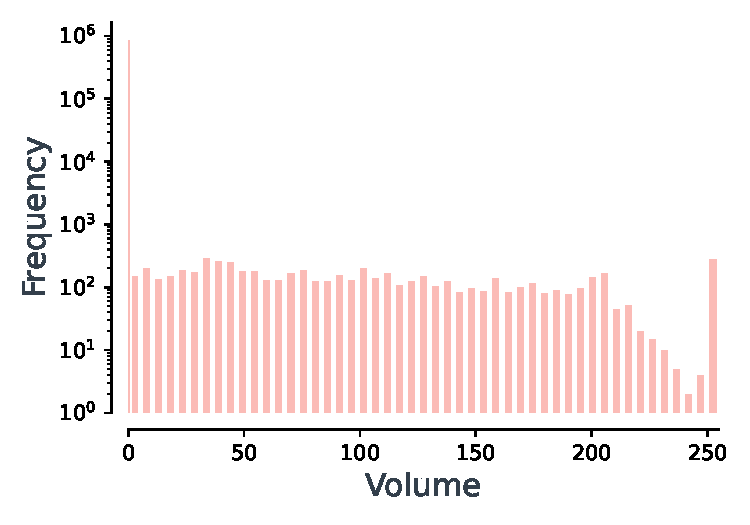
\includegraphics[width=0.9\textwidth]{./figures/volume.pdf}
         \caption{Histogram for data distribution for the volume.}
         \label{fig:volume}
    \end{minipage}
\end{figure}


\begin{figure}[!ht]
\noindent\hspace{0.5mm}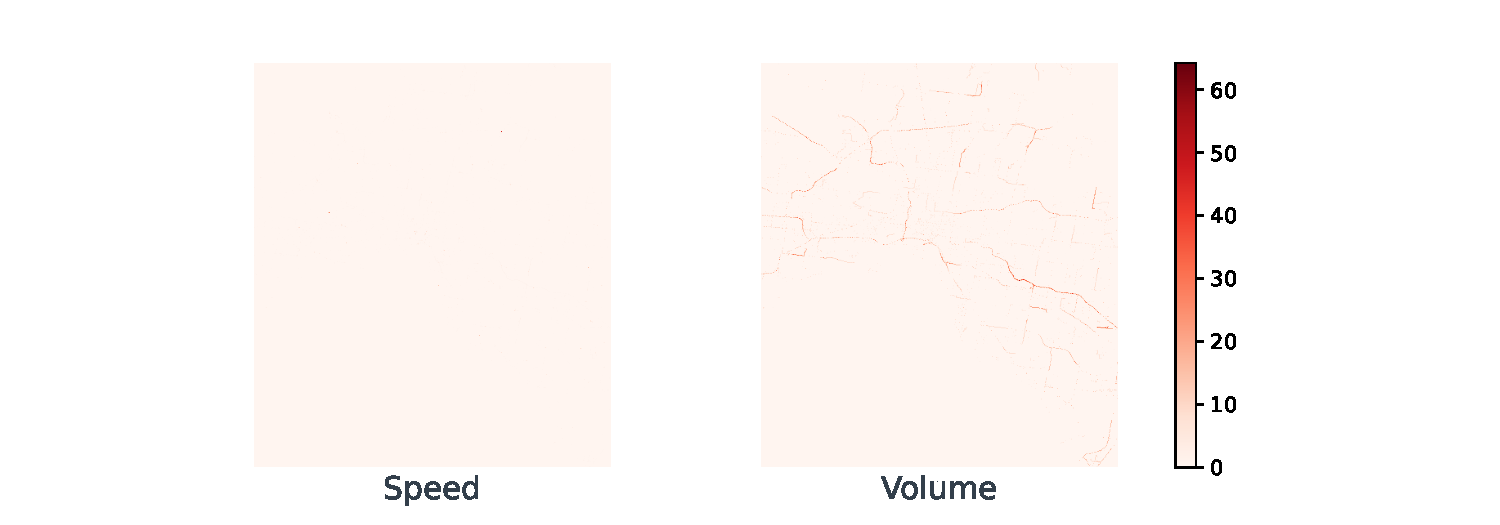
\includegraphics[width=0.9\textwidth]{./figures/heatmaps_speed_volume.pdf}
\caption{Heatmap of the snapshot for the (a) Speed; and (b) Volume. Note the first (very thin) bin with the null values.}
\label{fig:heatmap}
\end{figure}

\begin{table}[!h]
\centering
\resizebox{\textwidth}{!}{%
\begin{tabularx}{\textwidth}{XXXXX}
\hline
Channel \# & Mean & Median & Standard Deviation & Non-zero elements \% \\ \hline
0 (volume) & 0.0216 & 0.0000 & 0.2861 & 1.08\% \\
2 (volume) & 0.0141 & 0.0000 & 0.2794 & 0.84\% \\
4 (volume) & 0.0133 & 0.0000 & 0.6236 & 0.72\% \\
6 (volume) & 0.0118 & 0.0000 & 0.5957 & 0.62\% \\
1 (speed)  & 0.6758 & 0.0000 & 9.5058 & 0.73\% \\
3 (speed)  & 0.8655 & 0.0000 & 11.3655 & 0.82\% \\
5 (speed)  & 0.7419 & 0.0000 & 10.5863 & 0.71\% \\
7 (speed)  & 0.6149 & 0.0000 & 9.8281 & 0.60\% \\ \hline
\end{tabularx}%
}
\caption{Statistics for each channel in the specific snapshot}
\label{tab:data_analysis}
\end{table}

\subsection{Data processing}

Besides the disposal of the 2020 half of the original data, some other data processing transformations were realized. A significant part of the motivation for this processing step is to reduce the input data's size (or shape) to make the models trainable in a reasonable time, given the limited computational resources available. The first one of the transformations implemented was the collapse of the even (volume) and odd (speed) channels by taking the mean of the data in every channel. Therefore, we were left with two channels: the volume and average speed of the cars in the particular region.



%\begin{figure}[!ht]
%\noindent\hspace{0.5mm}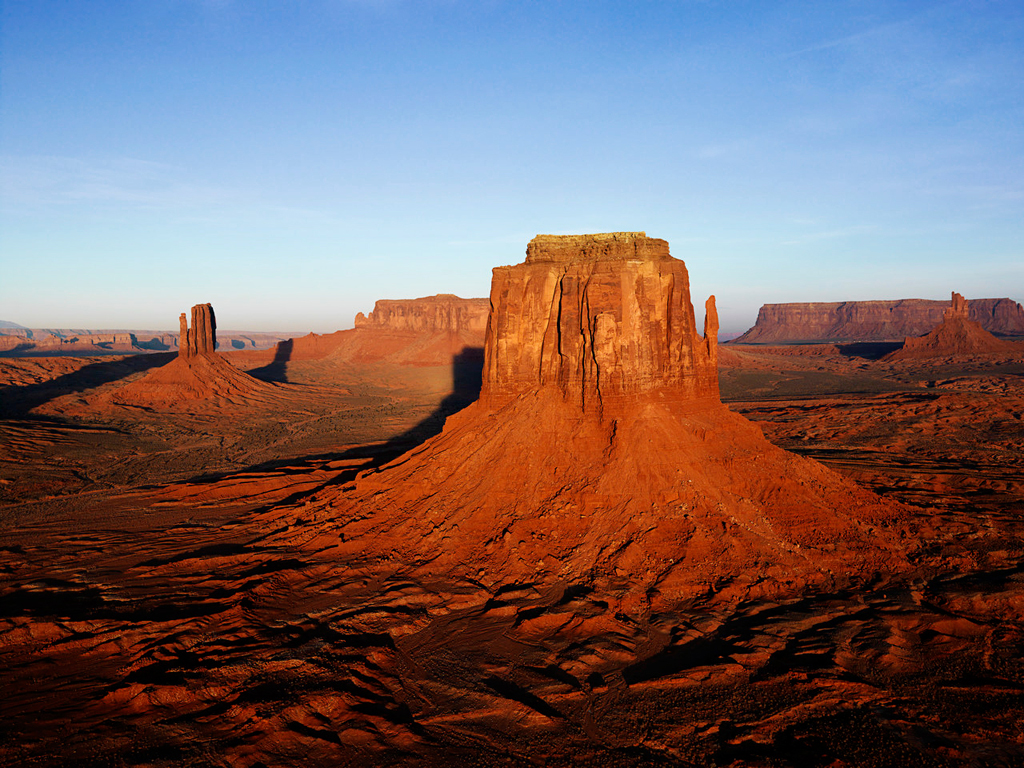
\includegraphics[width=12cm]{./resources/Desert.jpg}
%\caption{Title, Author}
%\end{figure}


\section{Model Outline}

The proposed model consists of three modules: a Feature Extraction Network, which is explained in Section \ref{sec:fen}; an Embedding Network, for which Section \label{sec:emb} is reserved; and a Prediction Network, the final layer, which is thoughtfully dissected in Section \ref{sec:pred}. This Section will explain the basis for the model and the overall architecture to be built.

\subsection{Task}
The field of Spatio-Temporal prediction is vast, allowing researchers to try different approaches to problems that may seem the same. This can be observed from the bibliography presented in the bibliographic revision. It's essential to clearly define the problem to be solved and the available information rigorously.

\begin{definition}\label{def:part}
A city $C$ is divided into a grid map of shape $W_{C}\times H_{C}$. Each partition $r_{i, j}$, with $0\leq i \leq W_C$ and $0\leq j \leq H_C$, is referred to as a region of $C$. The set containing all regions of the city is defined $R_C=\{r_{0, 0}, ..., r_{W_C, H_C}\}$.
\end{definition}

%\begin{definition}\label{def:conn}

%\end{definition}
\todo[inline]{maybe think about a connectivity definition, as we are dealing with graph networks and are using the edges as an argument for the ConvLSTM}

\begin{definition}\label{def:time}
The time range of available data of a city is divided into $T_{C}$  intervals of equal size: $t=[1, ..., t_{C}]$.
\end{definition}


\begin{definition}\label{def:ch}
For each region $r_{i, j}$, $N_{ch}$ data channels are available. These channels are the same for every city.
\end{definition}

By combining Definitions \ref{def:part}, \ref{def:time}, and \ref{def:ch} we can visualize the the 4D tensor of shape $(W_C, H_C, N_{ch}, T_C)$. Figure \ref{fig:data_tensor} shows a slice of this tensor. Each color represents a different channel, and each square of four colors represents a point in the 2D city grid. The stacked layers represent the time dimension.

\begin{definition} \label{def:dim}
A 4D tensor defines the data of a city $C$:
	\begin{equation}\label{eq:defdim}
		\mathcal{X}_C = \{x_{r, t}^{ch} | r \in R_C, t \in T_c, ch \in N_{ch}\}
	\end{equation}
\end{definition}

\begin{figure}[!ht]
\noindent\hspace{0.5mm}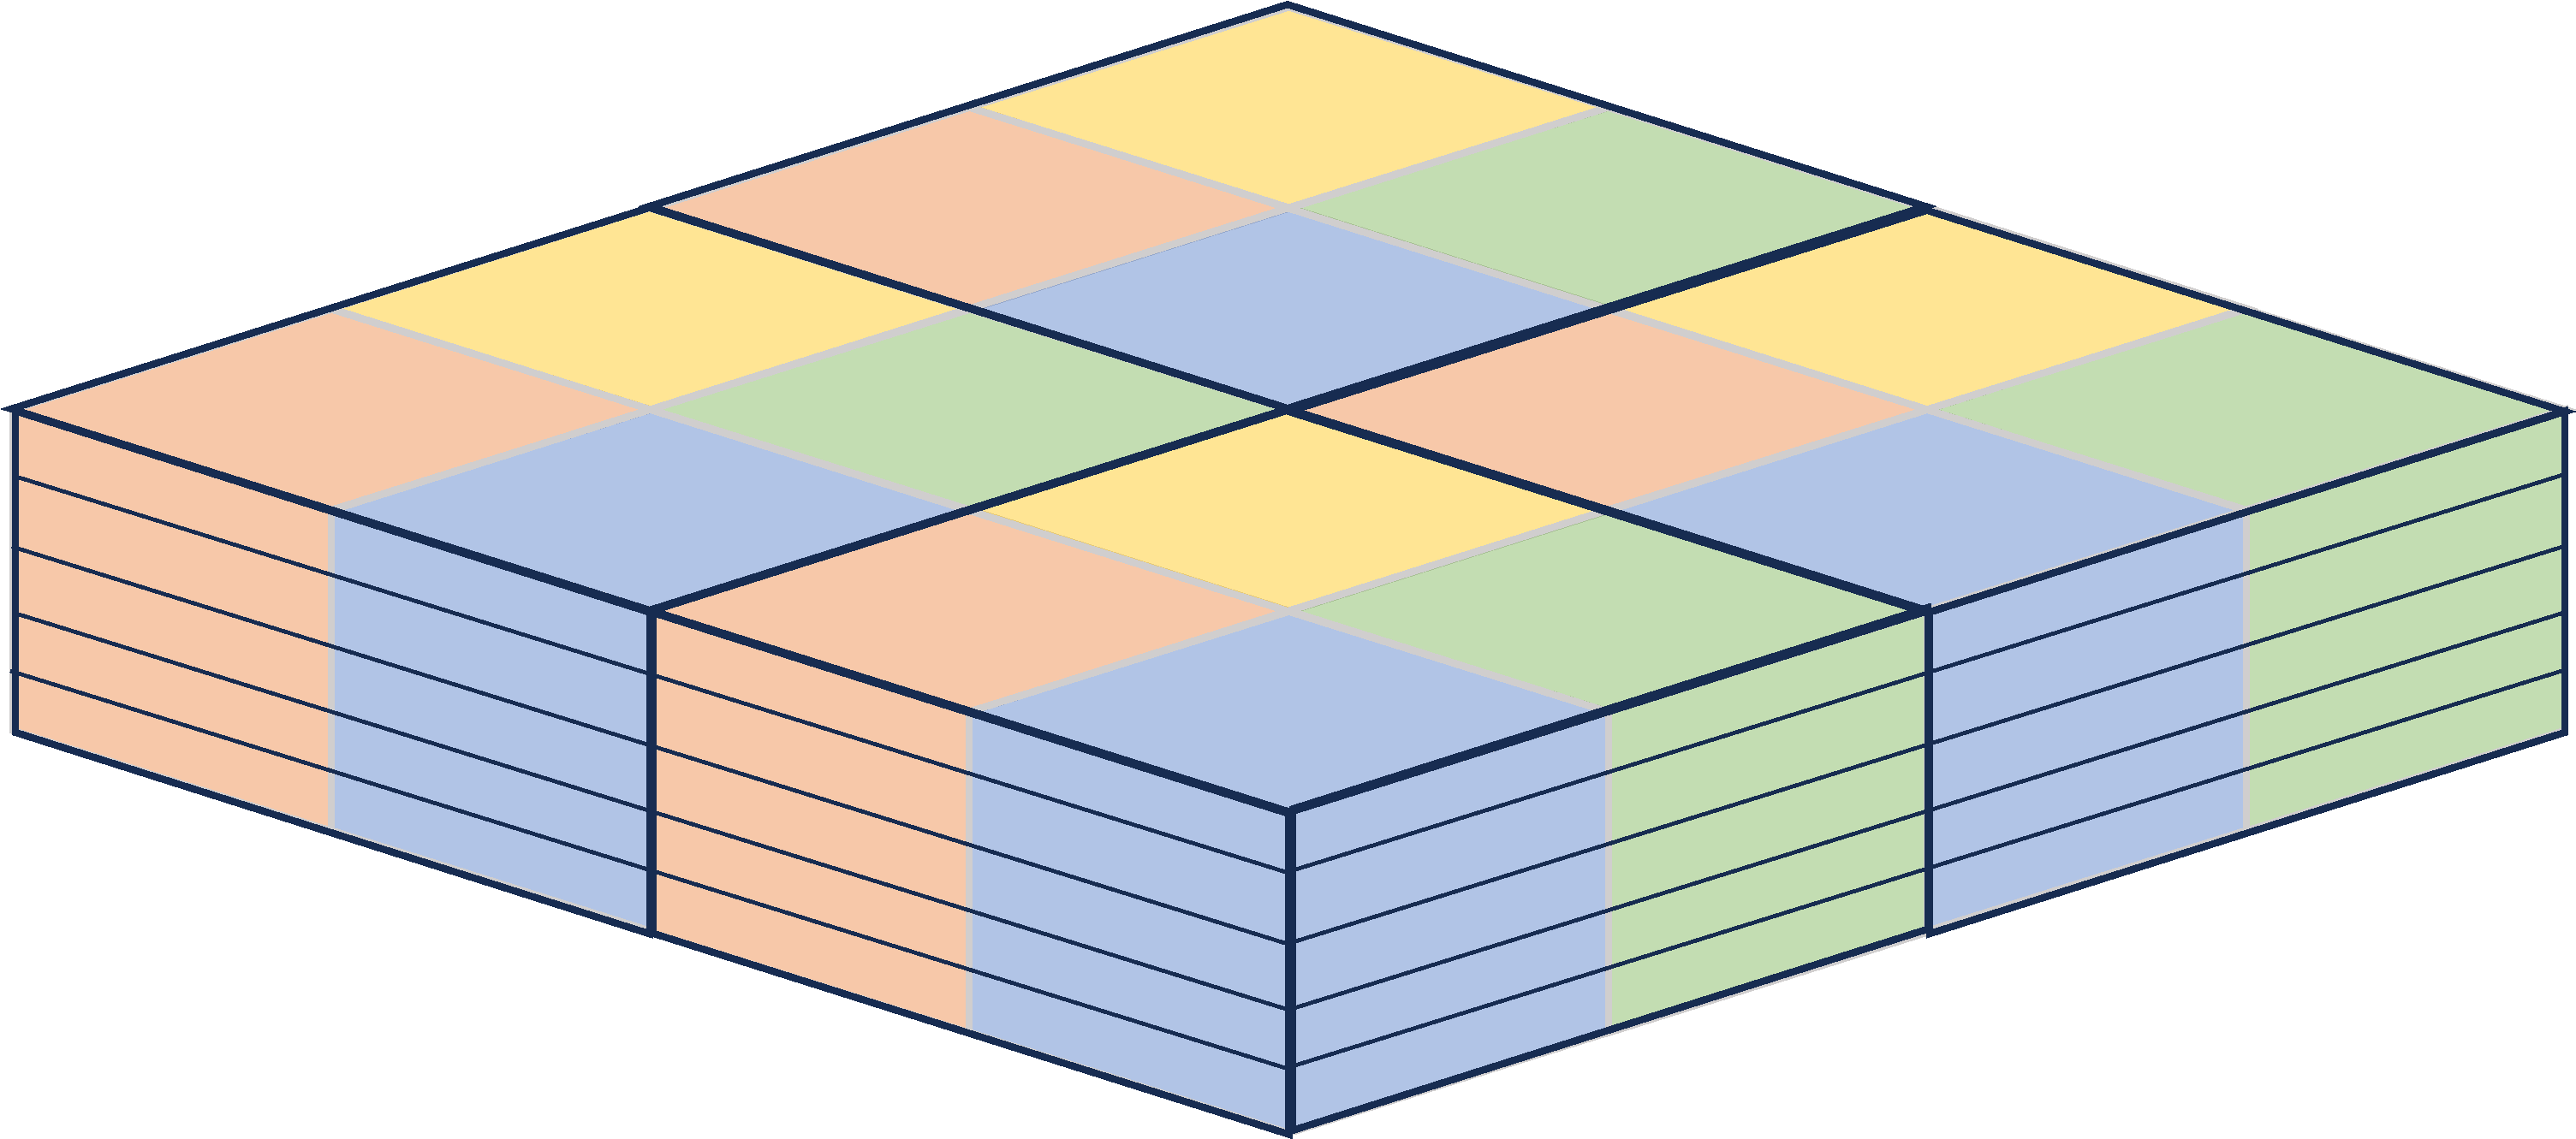
\includegraphics[width=0.6\textwidth]{./figures/data_tensor.pdf}
\caption{Visualization of the data (as a tensor).}
\label{fig:data_tensor}
\end{figure}

With these definitions, it's possible then to define Problem \ref{prob:tl}

\begin{problem} \label{prob:tl}
Given a data-scarce target city, $C_T$, and a set of $n$ data-rich source cities $\{C_{S1}, ..., C_{Sn}\}$, the problem proposed is to predict the value of the target city's data at $t_T+1$ with the historical data of the target city itself to that point and of the source cities:
	\begin{equation}\label{eq:probtl}
		\min_{\theta}\mathcal{L}(\tilde{\mathcal{X}}_{T, t_T + 1}, \mathcal{X}_{T, t_T + 1} )
	\end{equation}
	where
	\begin{equation}\label{eq:probtl2}
		\tilde{\mathcal{X}}_{T, t_T + 1} =  \theta(\mathcal{X}_{T, 1:t_T}, \{\mathcal{X}_{S1}, ..., \mathcal{X}_{Sn}\})
	\end{equation}
\end{problem}

Note that $ \mathcal{L}$ is the error criterion, which may vary depending on the actual data requirements. Note also that $t_{Sk} \gg t_T \forall k=1, ..., n$, indicating the target city's scarcity and the sources' richness.

\subsection{Proposed Architecture}

As explained at the beginning of this Section, the model comprises three parts: a Feature Extraction Network, an Embedding Network, and a Prediction Network. Figure \ref{fig:network_simplified} outlines the proposed architecture. Note that the individual modules will be developed and explained in their sections. Furthermore, three proposed losses are to be evaluated to train the model. The architecture adopted in this research draws upon the works of \cite{Wang202222, Wang20224695} as they proposed similar divisions in their models to transfer knowledge. Compared to their approach, we propose using a \gls{STGAE} as a mechanism to train the feature extractor and an adjacency matrix to represent connectivity between the regions.

\begin{figure}[!ht]
\noindent\hspace{0.5mm}\includegraphics[width=0.9\textwidth]{./figures/network_simplified.pdf}
\caption{Simplified version of the proposed model.}
\label{fig:network_simplified}
\end{figure}

\section{Feature Extraction Network} \label{sec:fen}

As the first layer of the model, the Feature Extraction Network receives an input of tensors from one or more source cities and from the target city and tries to extract, from these tensors, \gls{ST} features must be extracted to be used to train the Prediction Network. 

\subsection{Autoencoder}
 
 Selecting hyperparameters and fine-tuning an extractor are challenging tasks in constructing a model, as it's very difficult to observe causality between the change of a parameter and the change of the output due to the highly non-linear characteristics of these modules. As a result of these problems, the use of autoencoders for the feature extraction task has been proposed by \cite{Hinton2006}, and it's, as of today, a well-established paradigm in the \gls{ST} field. By conceptualizing the feature extraction process through the lens of an encoder, it becomes easier to verify its quality with the construction of a corresponding decoder. As the encoder maps the input data from its original vectorial space to a latent space, the decoder pursues the contrary operation, bringing back the data from the latent space to the original one. In an ideal scenario, a well-trained autoencoder will reconstruct the original data perfectly, guaranteeing the quality of the features extracted by the encoder.
 
More recently, \cite{fan2023spatiotemporal} implemented a \gls{STAE} by coupling \gls{GLU} layers for time convolution and Chebyshev convolution layers for spatial convolution. By interpolating two temporal layers by a spatial one, the authors extracted both spatial and temporal features. Additionally, using Chebyshev filters of relatively large sizes ($F=6$), the proposed autoencoder could properly derive features on both local and global scales.

In another paper, \cite{sabbaqi2022graph} proposes a generic framework for \gls{STGAE} with symmetric encoder-decoder architectures. The encoder finds a latent representation of the graph by applying graph convolutions, temporal downsampling layers, and activation functions. The decoder mirrors this behavior but uses temporal upsampling layers between the convolutions and activation functions. 
 
Figure \ref{fig:autoencoder} illustrates the architecture of the \gls{STGAE} utilized in our feature extraction framework. The encoder predominantly comprises a \gls{GConvLSTM} block responsible for the intricate task of extracting spatio-temporal features. It is followed sequentially by an activation function, batch normalization, a regularization dropout layer, and a  linear transformation layer. Very similarly, the decoder incorporates analogous components, adding a Sigmoid activation function preceding the output. This configuration leverages the data normalization previously applied, wherein the value range of all channels was linearly transformed from $[0, 255]$ to a unit interval $[0, 1]$.

\begin{figure}[!ht]
\noindent\hspace{0.5mm}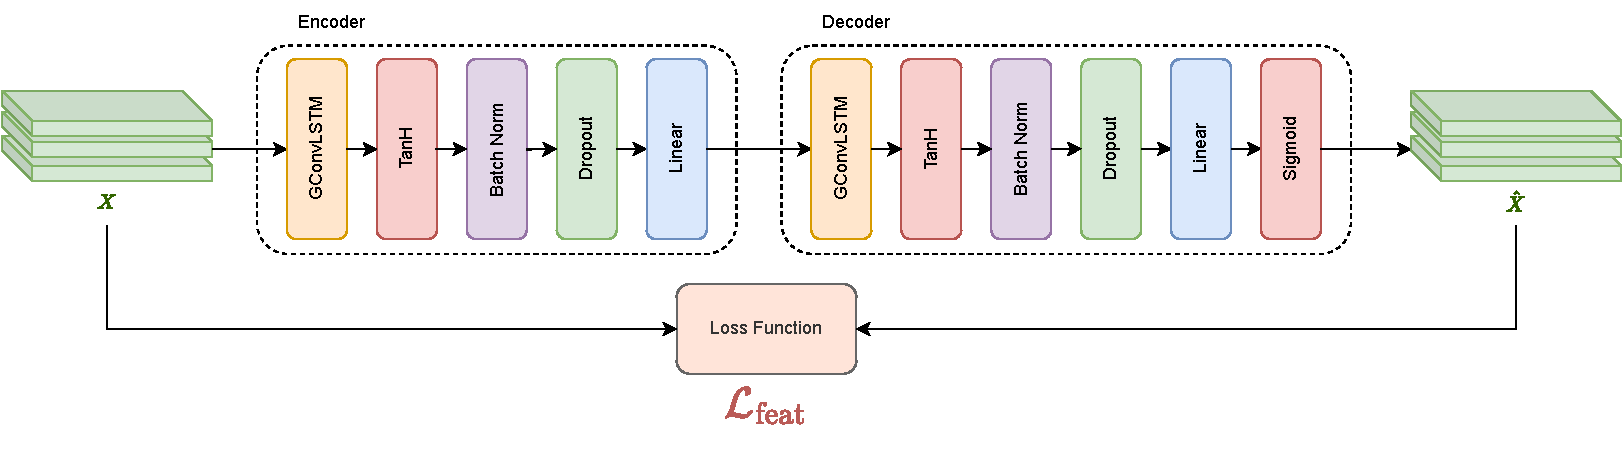
\includegraphics[width=0.9\textwidth]{./figures/Autoencoder.pdf}
\caption{Diagram representing the autoencoder as a combination of an encoder and a decoder.}
\label{fig:autoencoder}
\end{figure}

The \gls{GConvLSTM} cell, as implemented by \cite{rozemberczki2021pytorch}, and originally proposed by \cite{Seo_2018}, is parameterized by the number of input channels $N_{\text{in}}$, the number of output channels $N_{\text{out}}$, and the size of the Chebyshev polynomial filter $K$. The cell executes graph-based convolutions on the input tensor $x$, with the knowledge contained on the graph edge's descriptor tensor \texttt{edge\_index}, to yield the hidden state $h$ and the cell state $c$. These states are then propagated through the sequence for subsequent iterations, which are defined by the $k$ discrete temporal segments of which the input $x$ is composed. This enables the model to capture and encode the temporal dynamics of the data.

\begin{equation}
    \text{GConvLSTM}: \mathbb{R}^{D_1 \times D_2 \times \ldots \times D_N \times N_{\text{in}}} \rightarrow \mathbb{R}^{D_1 \times D_2 \times \ldots \times D_N \times N_{\text{out}}}
\end{equation}

Furthermore, as implemented in this layer, the order of the Chebyshev filter plays a pivotal role, as it defines the range of neighborhood aggregation. Specifically, it dictates how local neighborhoods are expanded around each node during the convolutional process. This in turn, influences the gradient computation during backpropagation, affecting both the receptive field and the capacity of the model to capture and integrate multi-hop relational information.




\subsection{Fine Tuning}

\section{Embedding Network} \label{sec:emb}

\section{Prediction Network} \label{sec:pred}


\section{Loss Functions} \label{sec:loss_func}

criterions